\documentclass{article}
\usepackage{float,amsmath}
\usepackage{graphicx}
\usepackage{color}
\usepackage[letterpaper,margin=0.75in]{geometry}
\usepackage{hyperref}

\usepackage{outlines}
\usepackage{enumitem}
\setenumerate[1]{label=\arabic*.}
\setenumerate[2]{label=\alph*.}
\setenumerate[3]{label=\arabic*.}
\setenumerate[4]{label=\roman*.}

\begin{document}

\author{HERA Team}
\title{HERA Rollout Plan}
\maketitle

\setcounter{section}{-1}
\section{Introduction}
HERA is operated in ``seasons'' that are denoted as:

\vspace{-0.25in}
\begin{table}[H]
\caption{HERA Operating Seasons}
\begin{tabular}{p{0.5in} p{2.2in} p{3.5in}} \hline
{\bf H0C} & season which ended in March 2017 & used the first 19 antennas (with their slightly wonky feeds). \\ \hline
{\bf H1C} & season which ended in April 2018    & start with 32, end with 71 with old feeds/architecture\\ \hline
{\bf H2C} & season to begin October 2018         & start with 59, end with 189 with new feeds/architecture\\ \hline
{\bf H3C} & season to begin August 2019           & 350 elements with new feeds/architecture \\ \hline
\end{tabular}
\end{table}

%A high-level schedule is shown in Fig. \ref{Fig:timeline}.   
Currently the project has recently completed H1C so this document provides a high-level roll-out discussion beginning for H2C.

%\begin{figure}[H]
%\includegraphics[width=\textwidth]{timeline.pdf} %under ProjectBook/Schedule
%\caption{High-level timeline.}
%\label{Fig:timeline}
%\end{figure}

\section{H2C}
The season will have two phases, H2C.A and H2C.B, which are summarized here:

\vspace{0.5cm}
\begin{tabular}{l l l l l l p{2.2in}}
 & \textbf{Date} & \textbf{\# ants} & \textbf{Chan/disc} & \textbf{Int} & \textbf{Total data} & \textbf{Comments} \\ \hline
H2C.A & 1 Oct 18 &  59-120   & 8192/1536 & 10 s&  X PB& Fringe-stopping hooks in, but not implemented.  Even-odd implemented. Walshing implemented. 187.5 MHz/122.1 kHz\\ \hline
H2C.B & 1 Jan 19 & 120-189 & 8192/3072 & 10 s& X PB & Fringe-stopping and baseline-dependent averaging implemented.  Goal to present data as same as H2C.A for DS users. 187.5 MHz/61.0 kHz\\ \hline
H3C    & 1 Aug 19 &  350       & 8192/6144 & 2  s&  X PB & all 187.5 MHz/30.5 kHz\\ \hline
\end{tabular}
\vspace{1cm}

The element roll-out is shown in Fig. \ref{Fig:rollout}.

\begin{figure}[H]
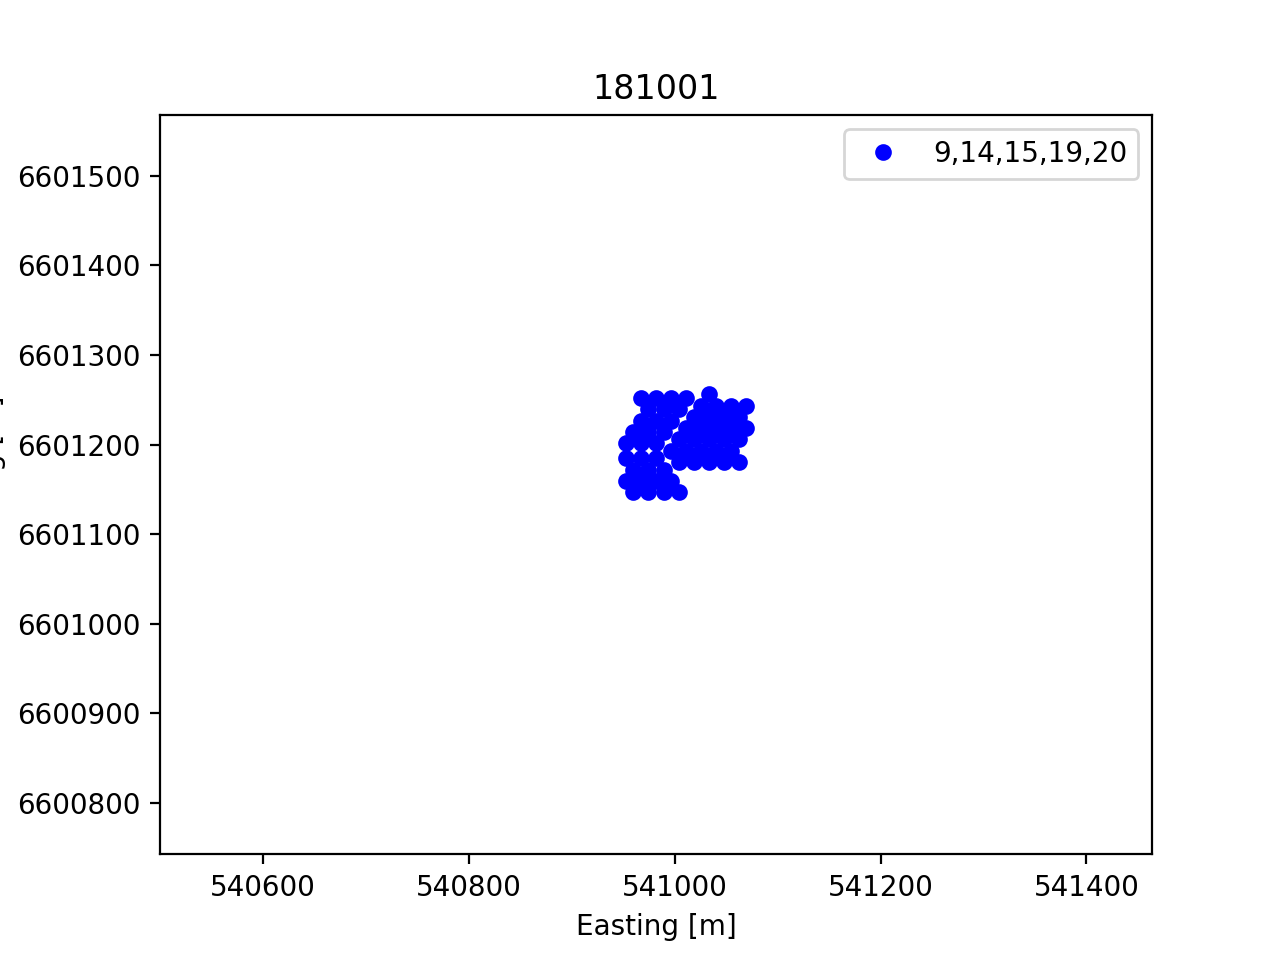
\includegraphics[width=0.36\textwidth]{cfg181001.png}
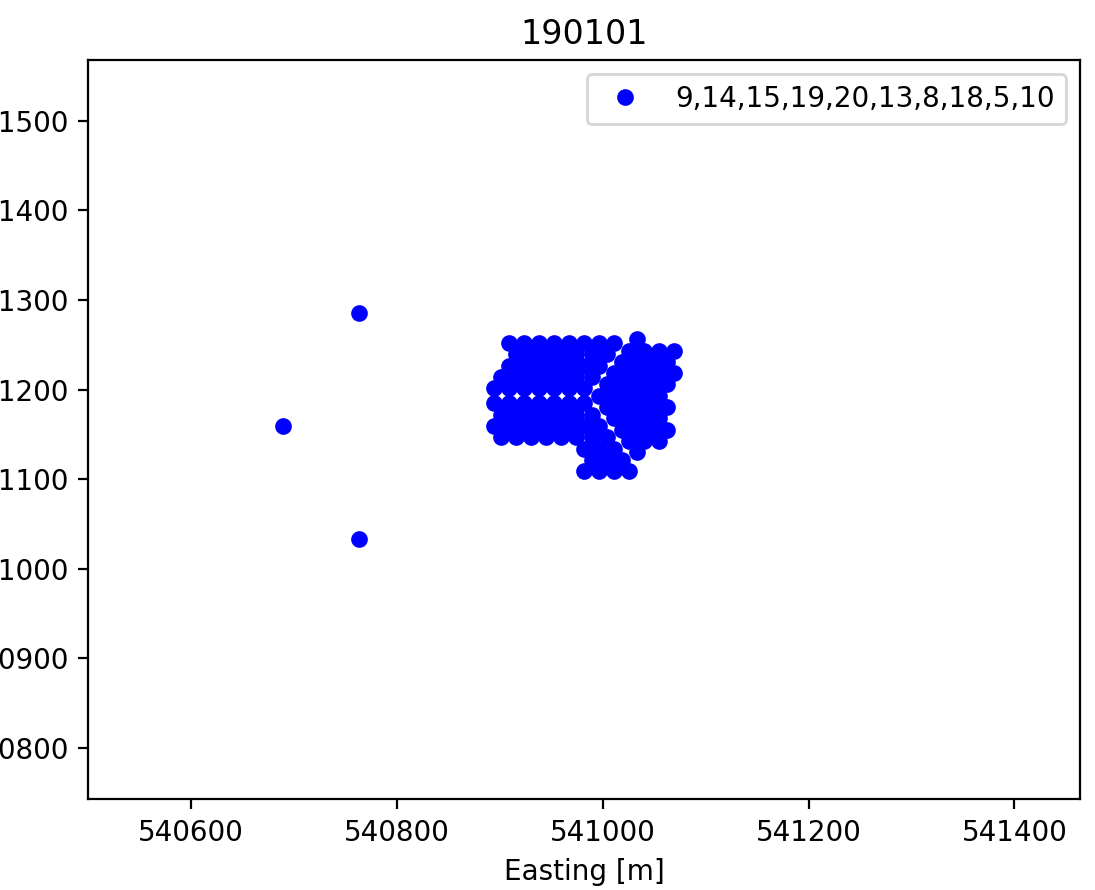
\includegraphics[width=0.36\textwidth]{cfg190101.png}
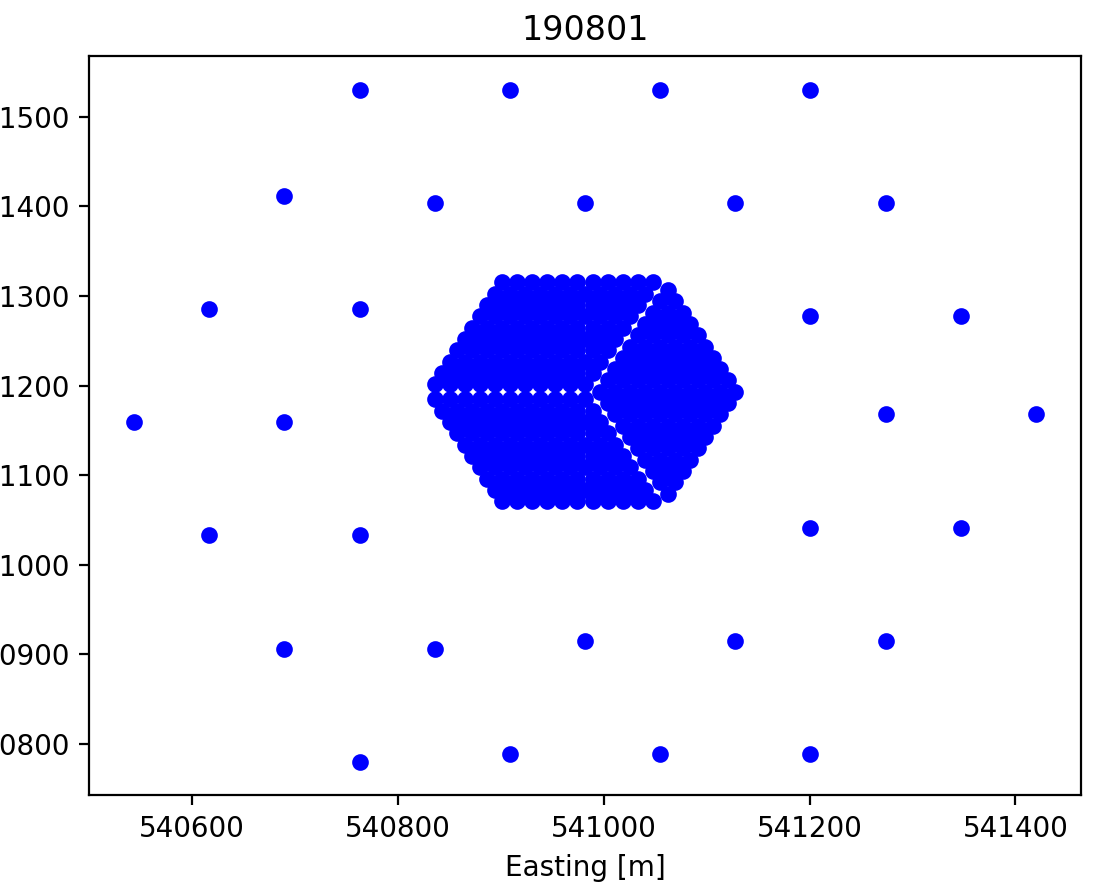
\includegraphics[width=0.36\textwidth]{ant_all.png}
\caption{Planned element rollout.  Left shows H2C.A comprising 59 elements by 1 Oct 2018.  Right shows H2C.B comprising 120 elements by 1 Jan 2019.  The legend lists the node numbers.}
\label{Fig:rollout}
\end{figure}

\end{document}
